\documentclass[aspectratio=169]{beamer}
\usepackage{pgfpages}
\setbeamertemplate{note page}[plain]

%enable notes
%\setbeameroption{show notes on second screen=right}
\usepackage[T1]{fontenc}
\usepackage[utf8]{inputenc}
\usepackage{lmodern}
\usepackage[french]{babel}
\usepackage{hyperref}
\usepackage{graphicx}
\usepackage{tikz}
\usepackage{makecell}
\usepackage{xcolor}
\usepackage{colortbl}
\usepackage[flushleft]{threeparttable}
\setbeamertemplate{note page}{\pagecolor{yellow!5}\insertnote}\usepackage{palatino}

\graphicspath{ {./img/} }

\newcommand{\TODO}{TODO:}
\newcommand*{\rot}{\rotatebox{90}}


\title{AIT --- Présentation}

% \titlegraphic{\includegraphics [height=.2\textheight] {logo_bacula.png}}
\author{
\includegraphics[height=2cm]{logo}\\Cassandre Wojciechowski \\ Gwendoline Dössegger \\ Noémie Plancherel \\ Gaby Roch}
\hypersetup{pdfauthor={G. Dössegger, N. Plancherel, G. Roch, C. Wojciechowski}}
\date{24 janvier 2022}

\begin{document}

\begin{frame}
  \titlepage
\end{frame}
%\begin{frame}
%  \tableofcontents
%\end{frame}

\section{Présentation générale}
\begin{frame}{Redis -- Présentation générale}
 \begin{itemize}
  \item Remote Dictionary Server
  \item Créateur Salvatore Sanfilippo
  \item Lancé en 2009 et continuellement mis à jour (dernière version 2021)
  \item Gratuit, opensource et multiplateforme
  \item Bonne documentation
 \end{itemize}
 \note{blabla}
\end{frame}

\section{Structure}
\begin{frame}{Structure}
\begin{itemize}
  \item SGBD NoSQL (clé-valeur)
  \item Types de données : string, object, listes, sets, ...
  \item In-memory database
  \item Ecriture en RAM en monothread 
\end{itemize}
 \note{ ...}
\end{frame}

\section{Database caching}
\begin{frame}{Database caching}
\begin{tikzpicture}[remember picture,overlay]
    \node[xshift=-3cm,yshift=-3cm] at (current page.north east){%
    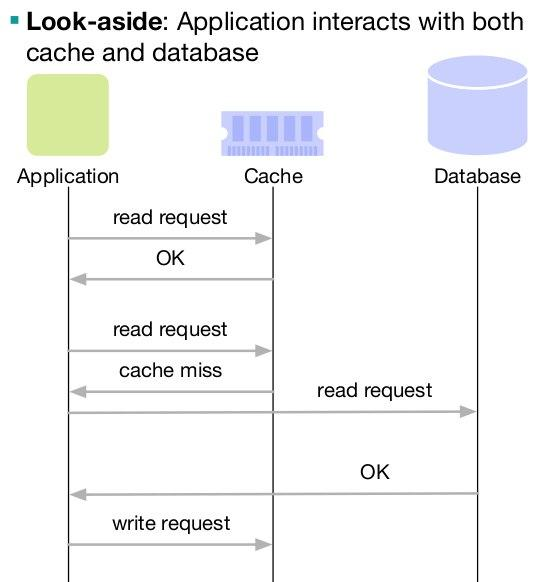
\includegraphics[width=5cm]{schema}};
\end{tikzpicture}
\begin{itemize}
  \item Look-Aside 
  \item Taille de mémoire maximale avec maxmemory
  \item Politique d'expulsion selon deux algorithmes \\ de gestion du cache
  \begin{itemize}
    \item LRU Algorithme approximatif
    \item LFU Algorithme
 \end{itemize}
\end{itemize}
 \note{ ...}
\end{frame}

\section{Démonstration}
\begin{frame}{Démonstration}
\TODO cas d'utilisation
\end{frame}

\section{Coûts}
\begin{frame}{Coûts}
\begin{center}

\begin{itemize}
    \item 2 versions: Open Source (gratuite) et Entreprise (payante)
    \item La version Entreprise permet une distribution globale de base de données Active-Active
    \item Elle assure une haute disponibilité (99,999\%)
    \item Ainsi qu'un support 24h/24 7j/7
    \item Redis Entreprise possède 2 versions
    \begin{itemize}
    \item Redis Entreprise Software
    \item Redis Entreprise Cloud
    \end{itemize}
    \item Possibilité de tester une version d'essai de 30 jours, sinon sur devis en fonction des besoins
\end{itemize}
\end{center}
\note{ ... }
\end{frame}

\section{Comparaison}
\begin{frame}{Comparaison}
 \begin{center}\small
  \begin{tabular}{|l|l|}
     \hline
      \textbf{Redis} & \textbf{Memcached} \\
     \hline
     \hline
        Plusieurs types de données & Pas de type de données  \\
        (string, hash, list, set, sorted set) & \\
     \hline
     Taille maximale de 512MB pour une valeur & Taille maximale de 1MB pour une valeur \\
     \hline
     Taille maximale de 512MB pour une clé  & Taille maximale de 250B pour une clé \\ 
     \hline
     Single-threaded & Multi-threaded \\
     (bonne scalabilité horizontale) & (scalabilité verticale facilitée) \\
     \hline
    Supporte 6 politiques d'expulsions & LRU comme seule politique d'expulsion  \\
     (no eviction, all keys LRU, ...) & \\
     \hline
     \end{tabular}
 \end{center}
 \note{ ... }
\end{frame}



\section{Avantages / inconvénients}
\begin{frame}{Avantages / inconvénients}
  \begin{center}
     \begin{tabular}{|l|l|}
     \hline
      \textbf{Avantages} & \textbf{Inconvénients} \\
     \hline
     \hline
        UI graphique + CLI & Principe clé-valeur \\
     \hline
     Variété de langages & Opérations simples \\
     \hline
     Variété de types de données & Prix de la scalabilité \\
     \hline
     Persistance & Single-threaded \\
     \hline
     Clustering & \\
     \hline
     Performances & \\
     \hline
     Documentation & \\
     \hline
     \end{tabular}

    \end{center}
\end{frame}

\section{Conclusion}
\begin{frame}{Conclusion}
 \begin{itemize}
  \item Utilisé par de grands acteurs (Twitter, Stackoverflow, Github)
  \item Flexibilité (langages, ...)
  \item Implémentation facile pouvant se faire très tôt
 \end{itemize}
\end{frame}

\begin{frame}{Questions ?}
\end{frame}


\end{document}
